\section{Versuchsauswertung}

\subsection{Versuch 1: Druckverluste}

Für den ersten Versuch wurde solarthermische Sammler eines Vakuumröhrenkollektors in den Versuchsstand eingebaut und der Druckverlust bei vier verschiedenen Volumenströmen gemessen. 
Mit Hilfe folgender Formel X und dem im Praktikum angegebenen $\zeta$-Werten wurden zusätzlich die Druckverluste für die eingestellten Volumenströme berechnet. Die experimentall ermittelten Druckverluste und die berechnten Druckversustwerte wurden in der folgenden Abbildung \ref{fig:drucksammler} abgebildet. 

	\begin{figure}[H]
	\centering
	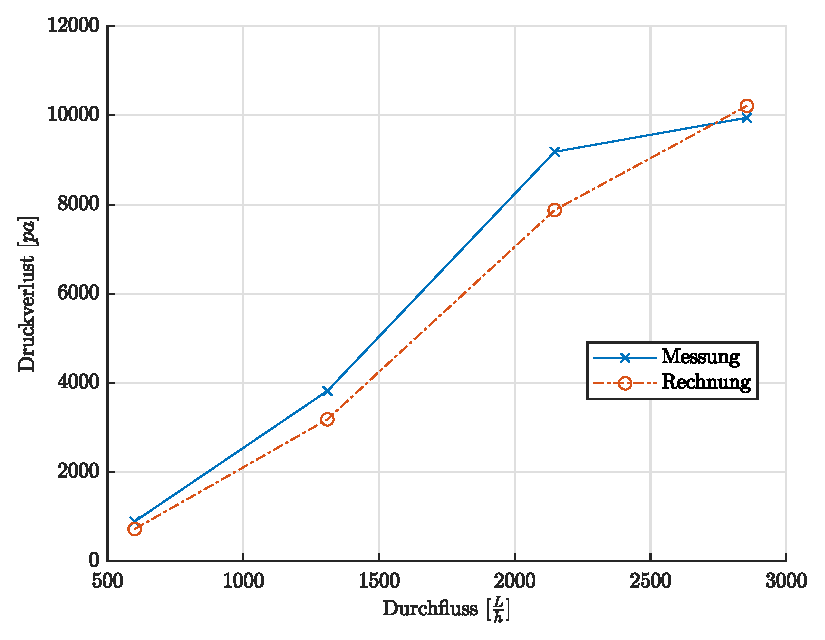
\includegraphics[height=0.3\textheight]{../DATA/dPPlot.eps}
	\caption[Druckverluste in Abhängigkeit der eingestellten Volumenströme für den Vakuumröhrensammler des Solarkollektors]{Druckverluste in Abhängigkeit der eingestellten Volumenströme für den Vakuumröhrensammler des Solarkollektors.}
	\label{fig:drucksammler}
	\end{figure}

Die experimentell ermittelten Druckverluste sind größer als die berechneten. Diese Abweichungen der Realität von den berechneten Daten kommt durch verschiedene Effekte zu stande. Die Bernoulli-Gleichung ist in ihrer Formulierung nur für stationäre Strömungen anzunehmen. Unter Anderem wird die Verkettung der den Hauptströmungsweg kreuzenden Röhren nicht berücksichtigt. Es wir bei der Anströmung jedes einzelnen Röhrchen von einer idealen stationären Anströmung ausgegangen, was in der gegebenen Anordnung nicht der Fall ist.

ZETA-WERTE!!!

\subsection{Versuch 2: Hydraulischer Abgleich}

\subsubsection{Berechnung der Ventilkennlinie für das Strangventil 2}
Für die Aufnahme der Ventilkennlinie wurden zunächst das Strangventils 2 vollständig geöffnet (Strangventil 1 und 3 vollständig geschlossen) und nach einer Volumenstromeinstellung von \SI{500}{\liter\per\hour} das Ventil schrittweise geschlossen. In der folgenden Abbildung \ref{fig:Ventil} wurde der Druckverlust in Abhängigkeit des Durchflusses aufgetragen. 

	\begin{figure}[H]
	\centering
	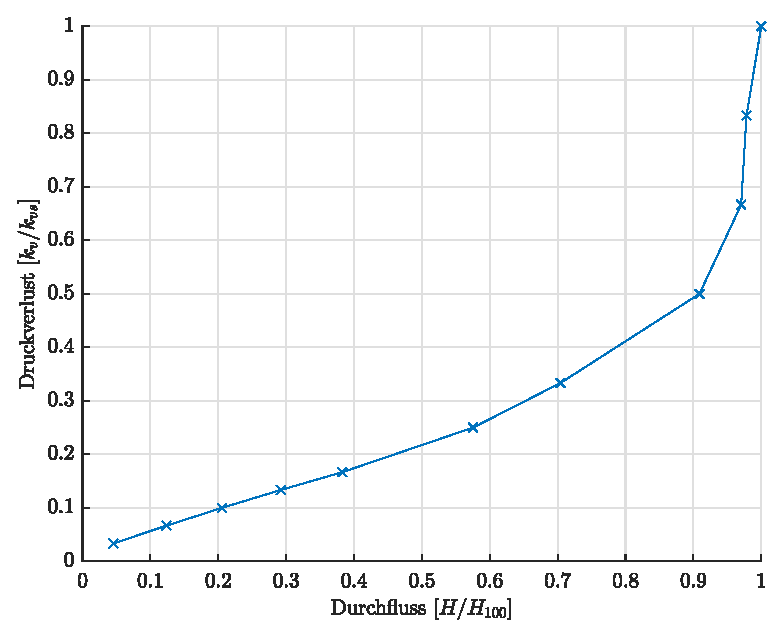
\includegraphics[height=0.4\textheight]{../DATA/Ventilkennlinie.eps}
	\caption[Ventilkennlinie des Strangventils 2]{Ventilkennlinie des Strangventils 2.}
	\label{fig:Ventil}
	\end{figure}

Wird das Ventil langsam zugeschraubt, verringert sich bis zu einer Ventilstellung von \num{3,0} der Durchfluss nur gering. Erst bei kleinen Ventilöffnungen kommt es zu einer überproportionalen Verringerung des Durchflusses. Die ermittelte Ventilkennlinie kommt der im Praktikumsskript gegebenen Kennlinie für das Ventil des Herstellers Vexve am nächsten. 

\subsubsection{Hydraulischer Abgleich durch Ausprobieren und mit Kompensationsmethode }

In dem Versuchsteil hydraulischer Abgleich durch Ausprobieren wurde versucht eine Schaltung von drei parallelen Strängen durch ausprobieren auf die selben Volumenströme zu bringen. Es wurde über das Pumpen- und Bypass-Ventil zunächst ein Volumenstrom von \SI{2000}{\liter\per\hour} bei vollständig geöffneten Strangventilen 1-4 eingestellt. Anschließend wurde der Volumenstrom des obersten Strangventils 1 als Soll-Wert angenommen und die anderen Ventile darauf eingestellt. Es wurden folgende Ventilstellungen und Volumenströme ermittelt. 

VERGLEICH der Methoden. 


D



\subsubsection{Tichelmannschaltung}

Bei der Schaltung nach Tichelmann wurde über das Pumpen- und Bypassventil wieder ein Volumenstrom von \SI{2000}{\liter\per\hour} eingestellt und anschießend die Volumenströme für alle drei Strangventile durch die Vortex-Durchfluss-Sensoren gemessen. In der folgenden Abbildung \ref{fig:Tichel} wurde der Druchfluss aller drei Sensoren der unterschiedlichen Stränge über einen Zeitraum von ca. \SI{60}{\second} gemessen.

\begin{figure}[H]
	\centering
	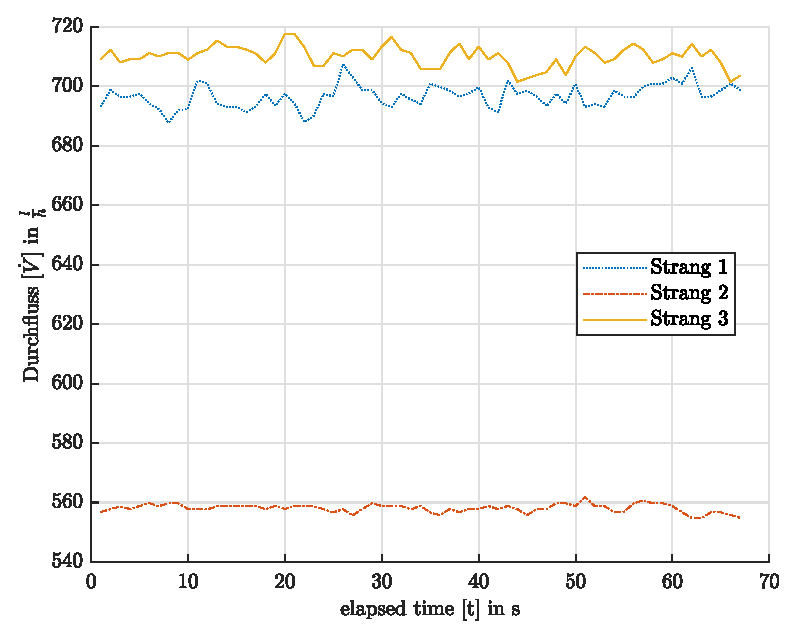
\includegraphics[height=0.4\textheight]{../DATA/Tichel.eps}
	\caption[Ventilkennlinie des Strangventils 2]{Ventilkennlinie des Strangventils 2.}
	\label{fig:Tichel}
\end{figure}

Durch eine Schaltung nach Tichelmann wird der theoretische Weg des Fluids durch alle drei Ventile gleich lang, sodass im Idealfall der Durchfluss für alle drei Ventile gleich sein sollte. In der Realität ist dies trotzdem nicht der Fall, da sich die Bauteile der Rohrleitung nicht ideal verhalten. In den Strängen 1 und 3 können annähernd gleiche Durchflussraten von \SI{700}{\liter\per\hour} bis \SI{710}{\liter\per\hour} erhalten werden. Für die Durchflussrate in Strang 2 wurde eine um ca. \SI{150}{\liter\per\hour} verringerte Durchflussrate ermittelt. Strangventil zwei wird im Gegensatz zu Strangventil 1 und 3 über zwei T-Stücke an die Tichelmannschaltung angeschlossen, die zu einen deutlich größeren Druckverlust am abzweigenden Strang des T-Stückes und damit zu einer geringeren Durchflussrate führen. Strang 1 und drei weisen hingegen nur Winkelstücke an den Kurven auf und unterscheiden sich untereinander dadurch weniger.  